% adapté de la RIG version française

\documentclass[french]{./sageo}

\confShortName{SAGEO'2017}
\confLongName{SAGEO'2017 - Rouen, 6-9 novembre 2017}

\usepackage[utf8]{inputenc} 
\usepackage[T1]{fontenc}
\usepackage{lmodern}
\usepackage{textcomp}
\usepackage{amsmath}
\usepackage{graphicx}
\usepackage{multirow}
\usepackage[noend]{algorithmic}
\usepackage[linesnumbered,ruled,vlined,boxed,commentsnumbered]{algorithm2e}

%% user packages and macros

\usepackage{ragged2e}





\firstpagenumber{1}


\title[Causalités Spatio-temporelles]{Identification de causalités dans des données spatio-temporelles}

\author[1,2]{Juste}{Raimbault}


% addresses are automatically numbered
\address{UMR CNRS 8504 Géographie-cités}
        {}
\address{UMR-T 9403 IFSTTAR LVMT}
        {juste.raimbault@polytechnique.edu}       

\resume{Cet article contribue à la compréhension des processus spatio-temporels fortement couplés, en proposant une méthode générique basée sur la causalité de Granger. Celle-ci est validée par l'identification robuste de régimes de causalité et de leur diagramme de phase pour un modèle de morphogenèse urbaine couplant croissance du réseau et de la densité. L'application au cas réel des projets de transport du Grand Paris démontre un lien entre les dynamiques territoriales, plus particulièrement socio-économiques et foncières, et la croissance anticipée du réseau. Nous discutons finalement des extensions possibles à d'autres échelles temporelles et spatiales.}


\motscles{Causalité Spatio-temporelle ; Interactions Réseaux-Territoires ; Morphogenèse Urbaine ; Grand Paris}

\keywords{Spatio-temporal Causality ; Network-territories Interactions ; Urban Morphogenesis ; Greater Paris}

\abstract{This paper contributes to the understanding of strongly coupled spatio-temporal processes by describing a generic method based on Granger causality. The method is validated by the robust identification of causality regimes and of their phase diagram for an urban morphogenesis model that couples network growth with density. The application to the real case study of Greater Paris transportation projects shows a link between territorial dynamics, more particularly of real estate and socio-economic, and the anticipated network growth. We finally discuss potential extensions to other temporal and spatial scales.}

\begin{document}

\maketitle

\newpage



%%%%%%%%%%%%%%%
\section{Introduction}
%%%%%%%%%%%%%%%



L'étude des processus spatio-temporels fortement couplés implique la prise en compte d'intrications entre ceux-ci généralement difficiles à isoler. Essence même des approches par la complexité, ces interactions qui sont à l'origine du comportement émergent d'un système font sens comme objet d'étude en lui-même, et une séparation des processus paraît alors contradictoire avec une vision intégrée du système. Dans le cas des systèmes territoriaux, l'exemple des interactions entre réseaux de transport et territoires est une excellente allégorie de ce phénomène : des méthodes isolant les ``effets structurants'' d'une infrastructure développées dans les années 70~\cite{bonnafous1974methodologies} se sont révélées par la suite de l'instrumentation politique et sans fondement empirique~\cite{offner1993effets}. Le débat est toujours d'actualité puisque la question se pose toujours par exemple pour la construction de lignes à grande vitesse~\cite{crozethalshs01094554}. La réalité des processus territoriaux est en fait bien plus compliqué qu'une simple relation causale entre la mise en place d'une infrastructure et les retombées sur le développement local, mais correspond bien d'une \emph{co-évolution} complexe~\cite{bretagnolletel00459720}. Sur le temps long et à grande échelle, certains effets de renforcement des dynamiques dans les systèmes de villes par l'insertion dans les réseaux, ont été mis en valeur par l'application de la Théorie Evolutive des Villes~\cite{espacegeo2014effets}, montrant que le démêlage est toutefois possible dans certains cas par une compréhension plus globale du système. A une autre échelle, toujours concernant les relations entre réseaux et territoires, on peut citer les liens entre pratiques de mobilité, étalement urbain et localisation des ressources dans un cadre métropolitain~\cite{cerqueira2017inegalites} qui s'avèrent tout autant complexes. Ce type de problématique est bien sûr présent dans d'autres domaines : en Economie Géographique, l'exemple des liens entre innovation, impacts locaux de la connaissance et aggregation des agents économiques est une illustration typiques de processus économiques spatio-temporels présentant des causalités circulaires difficiles à démêler~\cite{audretsch1996r}. Des méthodes spécifiques sont introduites, comme l'utilisation d'instruments statistiques comme par~\cite{aghion2015innovation} dans lequel l'origine géographique des membres du Bureau du Congrès américain attribuant les subventions locales est une bonne variable instrumentale pour lier caractère innovant et inégalités des plus haut salaires, et permet de montrer que la correlation significative entre les deux est en fait une causalité de l'innovation sur les inégalités.


Le couplage fort spatio-temporel implique généralement l'introduction de la notion de causalité, à laquelle la géographie s'est toujours intéressée : \cite{loi1985etude} montre que les questions fondamentales que se pose la géographie théorique récente (isolation des objects, lien entre espace et structures causales, etc.) étaient déjà présentes dans la géographie classique de Vidal. \cite{claval1985causalite} critique d'ailleurs les nouveaux déterminismes ayant émergé, notamment celui proposé par certains tenants de l'analyse systémique : dans ses débuts, cette approche héritait de la cybernétique et donc d'une vision réductionniste impliquant un déterminisme même dans une formulation probabiliste. Claval note que des travaux contemporains à son écriture devraient permettre de capturer la complexité qui fait la particularité des décisions humaines : l'école de Prigogine et la Théorie des Catastrophes de Thom. Ce point de vue est remarquablement visionnaire, puisque comme le rappelle Pumain dans \cite{pumain2003approche}, le glissement de l'analyse des systèmes à l'auto-organisation puis à la complexité a été long et progressif, et ces travaux ont été fondamentaux pour le permettre. François Durand-Dastès résume cette situation plus récemment dans \cite{durand2003geographes}, en appuyant l'importance des bifurcations et de la dépendance au chemin lors des instants initiaux de la constitution du système qu'il désigne par \emph{systèmogenèse}. % note : here we could introduce morphogenesis, form as system structure, linked to circular causalities ; topology and dynamical systems in network propagation (paper Nature Networks). Too far, but keep in mind for further work ?
Ce type de dynamique complexe implique généralement une co-évolution des composantes du système, qu'on peut interpréter comme des causalité circulaires entre processus : la question de pouvoir les identifier est donc cruciale au regard de la notion de causalité pour la géographie complexe contemporaine.

Les régimes sous lesquels des identifications de causalité sont cohérentes ne sont pas identifiés de manière évidente. Ceux-ci dépendront des définition utilisées, de la même manière que les méthodes à disposition pour lesquelles nous pouvons donner quelques illustrations. \cite{liu2011discovering} propose la detection de relations spatio-temporelles entre perturbations des flots de trafic, introduisant une définition particulière de la causalité basé sur une correspondance de points extrêmes. Les algorithmes associés sont toutefois spécifiques et difficilement applicables à des types de systèmes différents. L'utilisation des correlations spatio-temporelles a été démontrée comme ayant dans certains cas un fort pouvoir prédictif pour les flots de traffic~\cite{min2011real}. Egalement dans le domaine des transports et de l'usage du sol, \cite{xie2009streetcars} applique une analyse par causalité de Granger, qu'on pourra interpréter comme une corrélation retardée, pour montrer dans un cas particulier que la croissance du réseau induit le développement urbain et est elle-même tirée par des externalités comme les habitudes de mobilité. Les neurosciences ont développé de nombreuses méthodes répondant à des problématiques similaires. \cite{luo2013spatio} définit une causalité de Granger généralisée prenant en compte la non-stationnarité et s'appliquant à des régions abstraites issues d'imagerie fonctionnelle. Ce genre de méthode est également développée en Vision par Ordinateur, comme l'illustre \cite{ke2007spatio} qui exploite les correlations spatio-temporelles de formes et de flux dans des successions d'images pour classifier et reconnaître des actions. Les applications peuvent être très concrète comme la compression de fichier videos par extrapolation des vecteurs de mouvement~\cite{chalidabhongse1997fast}. Dans l'ensemble de ces cas, l'étude des correlations spatio-temporelles rejoint les notions faibles de causalité vues précédemment. Cette contribution cherche à explorer la possibilité d'une méthode analogue pour des données spatio-temporelles présentant a priori des causalités circulaires complexes, et donc de tenter l'exercice d'équilibriste de concilier un certain niveau de simplicité et de caractère opérationnel à une prise en compte de la complexité. Nous introduisons ainsi une méthode d'analyse des correlations spatio-temporelles similaire à une causalité de Granger estimée dans le temps et l'espace, dont la robustesse est démontrée systématiquement par l'application à un modèle de simulation complexe de morphogenèse urbaine et par l'isolation de régimes de causalités distincts dans l'espace des phases du modèle. Notre contribution inclut également l'application à un cas d'étude empirique, ce qui la positionne à l'interface des domaines de la méthodologie, de la modélisation et de l'empirique.


La suite de cette article est organisée de la façon suivante : le cadre générique de la méthode proposée est décrit dans la section suivante. Nous l'appliquons ensuite à un jeu de données synthétiques afin de la valider partiellement et de tester ses potentialité, ce qui permet de l'appliquer ensuite au cas d'étude réel des réseaux de transport du Grand Paris. Nous discutons finalement la proximité avec d'autres méthodes existantes et des développements possibles.



%%%%%%%%%%%%%%%
\section{Méthode}
%%%%%%%%%%%%%%%

% some kind of smoothing has to be introduced, either as preprocessing or as part of the optimization process (at least for first observed behavior on synthetic data. maybe it is typical of the model ?) -> similar to take into account spatial autocorrelation ? (not exactly, but close)
% - formalize mean estimator on repetitions, compare it to a direct estimator (// computation or aggregated data ?) -> OK, no need to explicit estimator in the generic part

Nous formalisons ici de manière générique la méthode, basée sur un test similaire à la causalité de Granger, pour tenter d'identifier des relations causales dans des systèmes spatiaux. Soit $X_j(\vec{x},t)$ des processus aléatoires spatiaux unidimensionnels, se réalisant dans le temps et l'espace. On se donne un ensemble d'unités spatiales fondamentales $(u_i)$ qui peuvent être par exemple les cellules d'un raster ou un pavage quelconque de l'espace géographique. On suppose l'existence de fonctions $\Phi_{i,j}$ permettant de faire correspondre les réalisations de chaque composante aux unités spatiales, possiblement par une première agrégation locale. Une réalisation d'un système est donnée par un ensembles de trajectoires pour chaque processus $x_{i,j,t}$, et on pourra noter un ensemble de réalisations $x^{(k)}_{i,j,t}$ (accessibles dans le cas d'un modèle de simulation par exemple, ou par hypothèse de comparabilité de sous-systèmes territoriaux dans des cas réels). On suppose disposer d'un estimateur de correlation $\hat{\rho}$ s'exerçant dans le temps, l'espace et les répétitions, i.e. $\hat{\rho}\left[X,Y\right] = \hat{\mathbb{E}}_{i,t,k}\left[XY\right] - \hat{\mathbb{E}}_{i,t,k}\left[X\right]\hat{\mathbb{E}}_{i,t,k}\left[Y\right]$. Il est important de noter ici l'hypothèse de stationnarité spatiale et temporelle, qui peut toutefois aisément se relâcher dans le cas d'une stationnarité locale. D'autre part, l'autocorrelation spatiale n'est pas explicitement incluse, mais est prise en compte soit par l'agrégation initiale si l'échelle caractéristique des unités est plus grande que celle des effets de voisinage, soit par un estimateur spatial adéquat (statistiques spatiales pondérées de type \emph{GWR}~\cite{brunsdon1998geographically} par exemple). Cela nous permet de définir la correlation retardée par

\begin{equation}
\rho_{\tau}\left[X_{j_1},X_{j_2}\right] = \hat{\rho}\left[x^{(k)}_{i,j_1,t - \tau},x^{(k)}_{i,j_2,t}\right]
\end{equation}

La corrélation retardée n'est pas directement symétrique, mais on a de manière évidente $\rho_{\tau}\left[X_{j_1},X_{j_2}\right] = \rho_{-\tau}\left[X_{j_2},X_{j_1}\right]$. On applique alors cette mesure de manière simple : si $\textrm{argmax}_{\tau} \rho_{\tau}\left[X_{j_1},X_{j_2}\right]$ ou $\textrm{argmin}_{\tau} \rho_{\tau}\left[X_{j_1},X_{j_2}\right]$ sont ``clairement définis'' (les deux pouvant l'être simultanément), leur signe donnera alors le sens de la causalité entre les composantes $j_1$ et $j_2$ et leur valeur absolue le retard de propagation. Les critères de significativité dépendront du cas d'application et de l'estimateur utilisé, mais peuvent par exemple inclure la significativité du test statistique (test de Fisher dans le cas d'un estimateur de Pearson), la position des bornes d'un intervalle de confiance à un niveau donné, ou même un seuil exogène $\theta$ sur $\left|\rho_{\tau}\right|$ pour forcer un certain degré de correlation. 










%%%%%%%%%%%%%%%
\section{Résultats}
%%%%%%%%%%%%%%%


%%%%%%%%%%%%%%%
\subsection{Données Synthétiques}



%%%%%%%%%%%%%%%
\begin{figure*}[h]
\centering
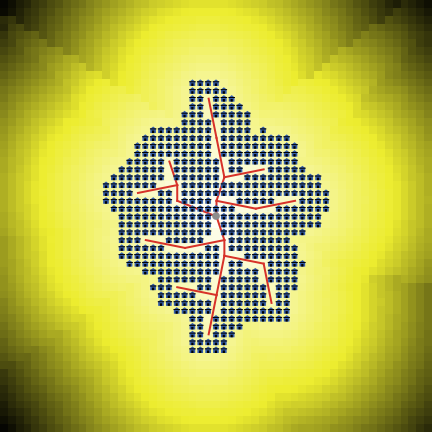
\includegraphics[width=3.9cm]{figures/ex_60_wdens0_wroad1_wcenter1_seed272727}
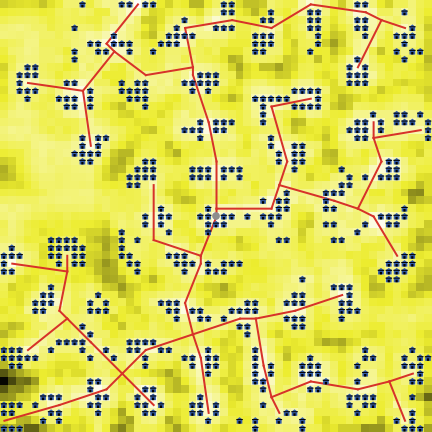
\includegraphics[width=3.9cm]{figures/ex_60_wdens1_wroad1_wcenter0_seed272727}
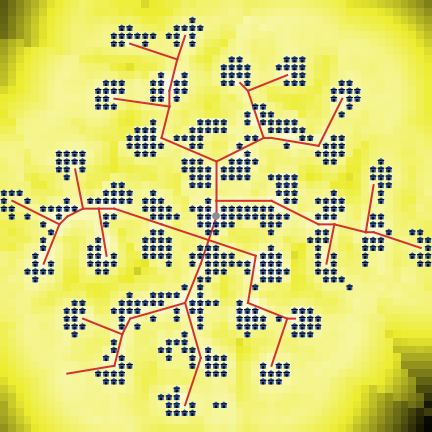
\includegraphics[width=3.9cm]{figures/ex_60_wdens1_wroad1_wcenter1_seed272727}\\\vspace{0.2cm}
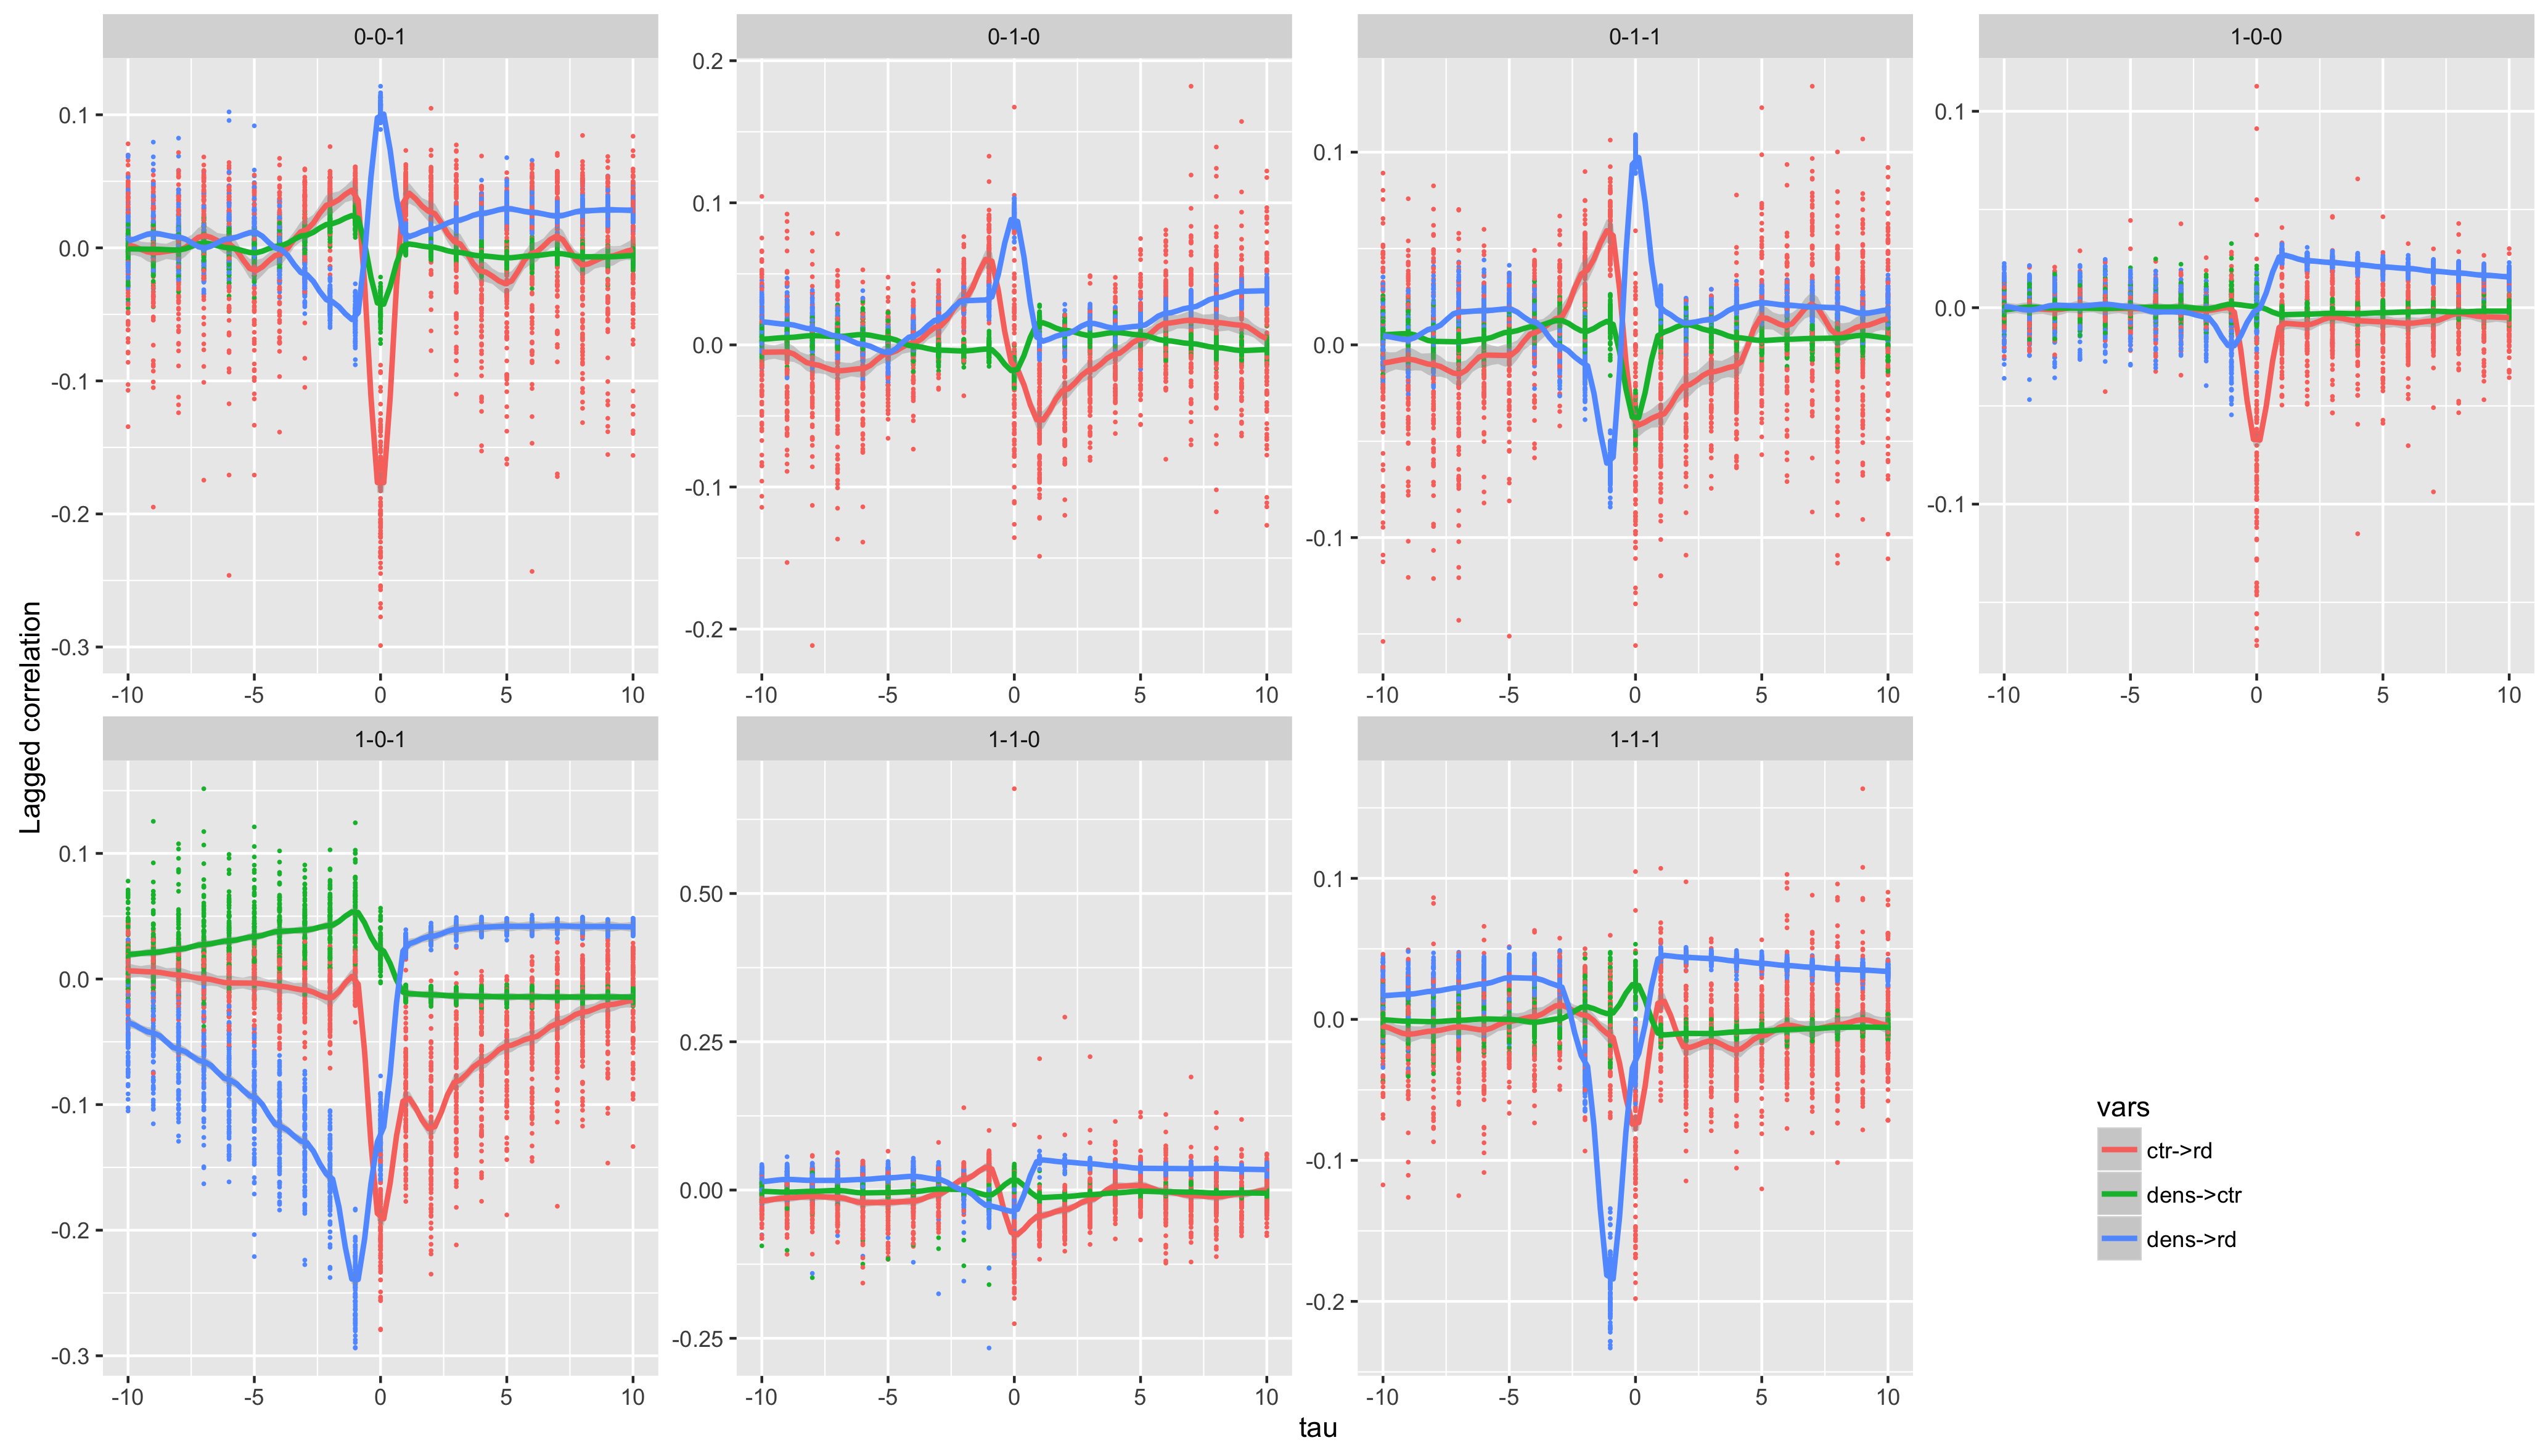
\includegraphics[width=12cm]{figures/laggedcorrs_facetextreme}
\caption{\textbf{Correlations dans le modèle RDB} \textbf{(Première ligne)} Exemples de configurations finales variées, obtenues avec $(w_{d},w_{c},w_{r})$ valant respectivement $(0,1,1)$,$(1,0,1)$, et $(1,1,1)$. \textbf{(Deuxième ligne)} Corrélations retardées, pour chaque combinaison des paramètres, en fonction du retard $\tau$. Les différentes couleurs correspondent à chaque couple de variables : distance au centre (\texttt{ctr}), densité (\texttt{dens}) et distance au réseau (\texttt{rd}). Les points montrent l'étendue sur l'ensemble des répétitions du modèle (estimateurs sur $i$ et $t$).}
\label{fig:exrdb}
\end{figure*}
%%%%%%%%%%%%%%%



%%%%%%%%%%%%%%%
\begin{figure*}[h]
\centering
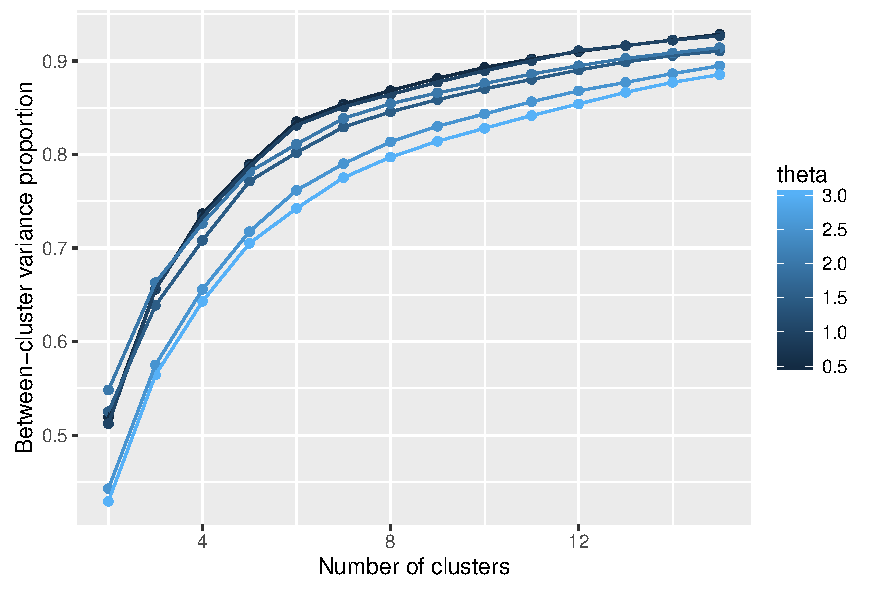
\includegraphics[width=3.9cm,height=3.2cm]{figures/ccoef-knum_valuesFALSE_theta05-3.pdf}
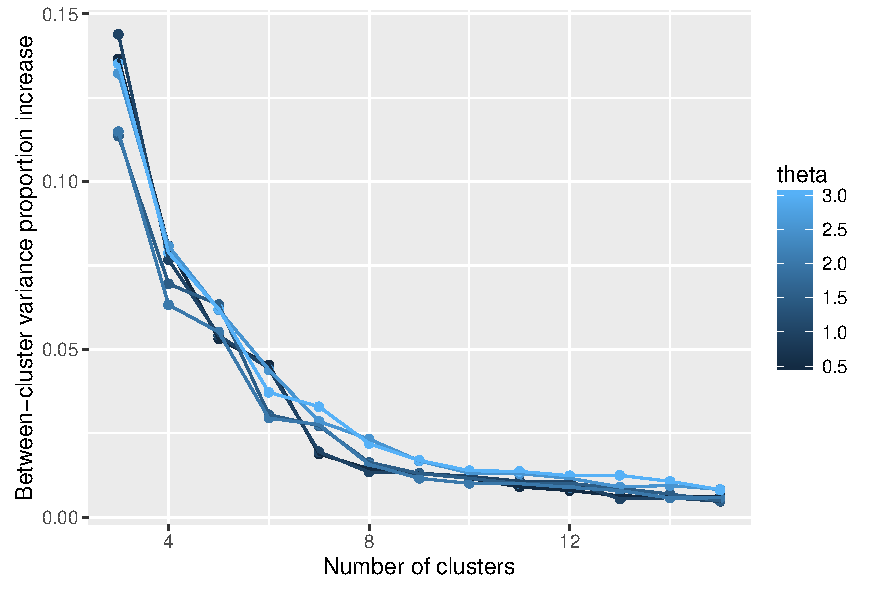
\includegraphics[width=3.9cm,height=3.2cm]{figures/dccoef-knum_valuesFALSEtheta05-3.pdf}
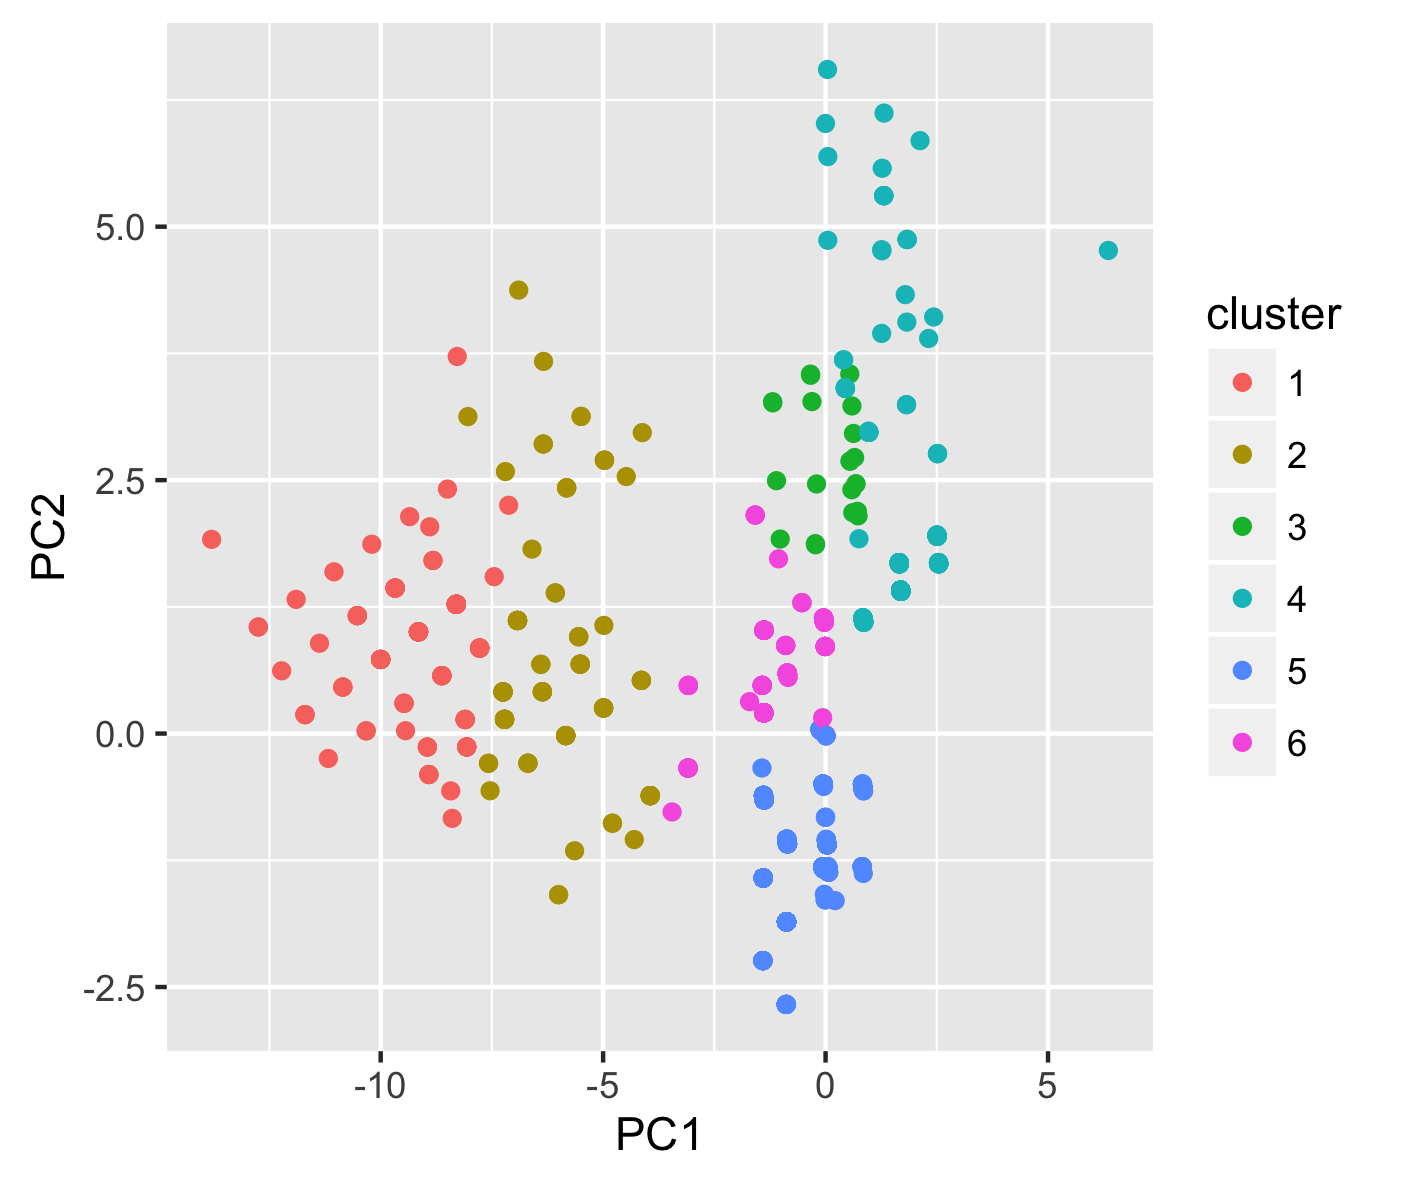
\includegraphics[width=3.9cm,height=3.2cm]{figures/clusters-PCA-features_valuesFALSEtheta2_k6}\\
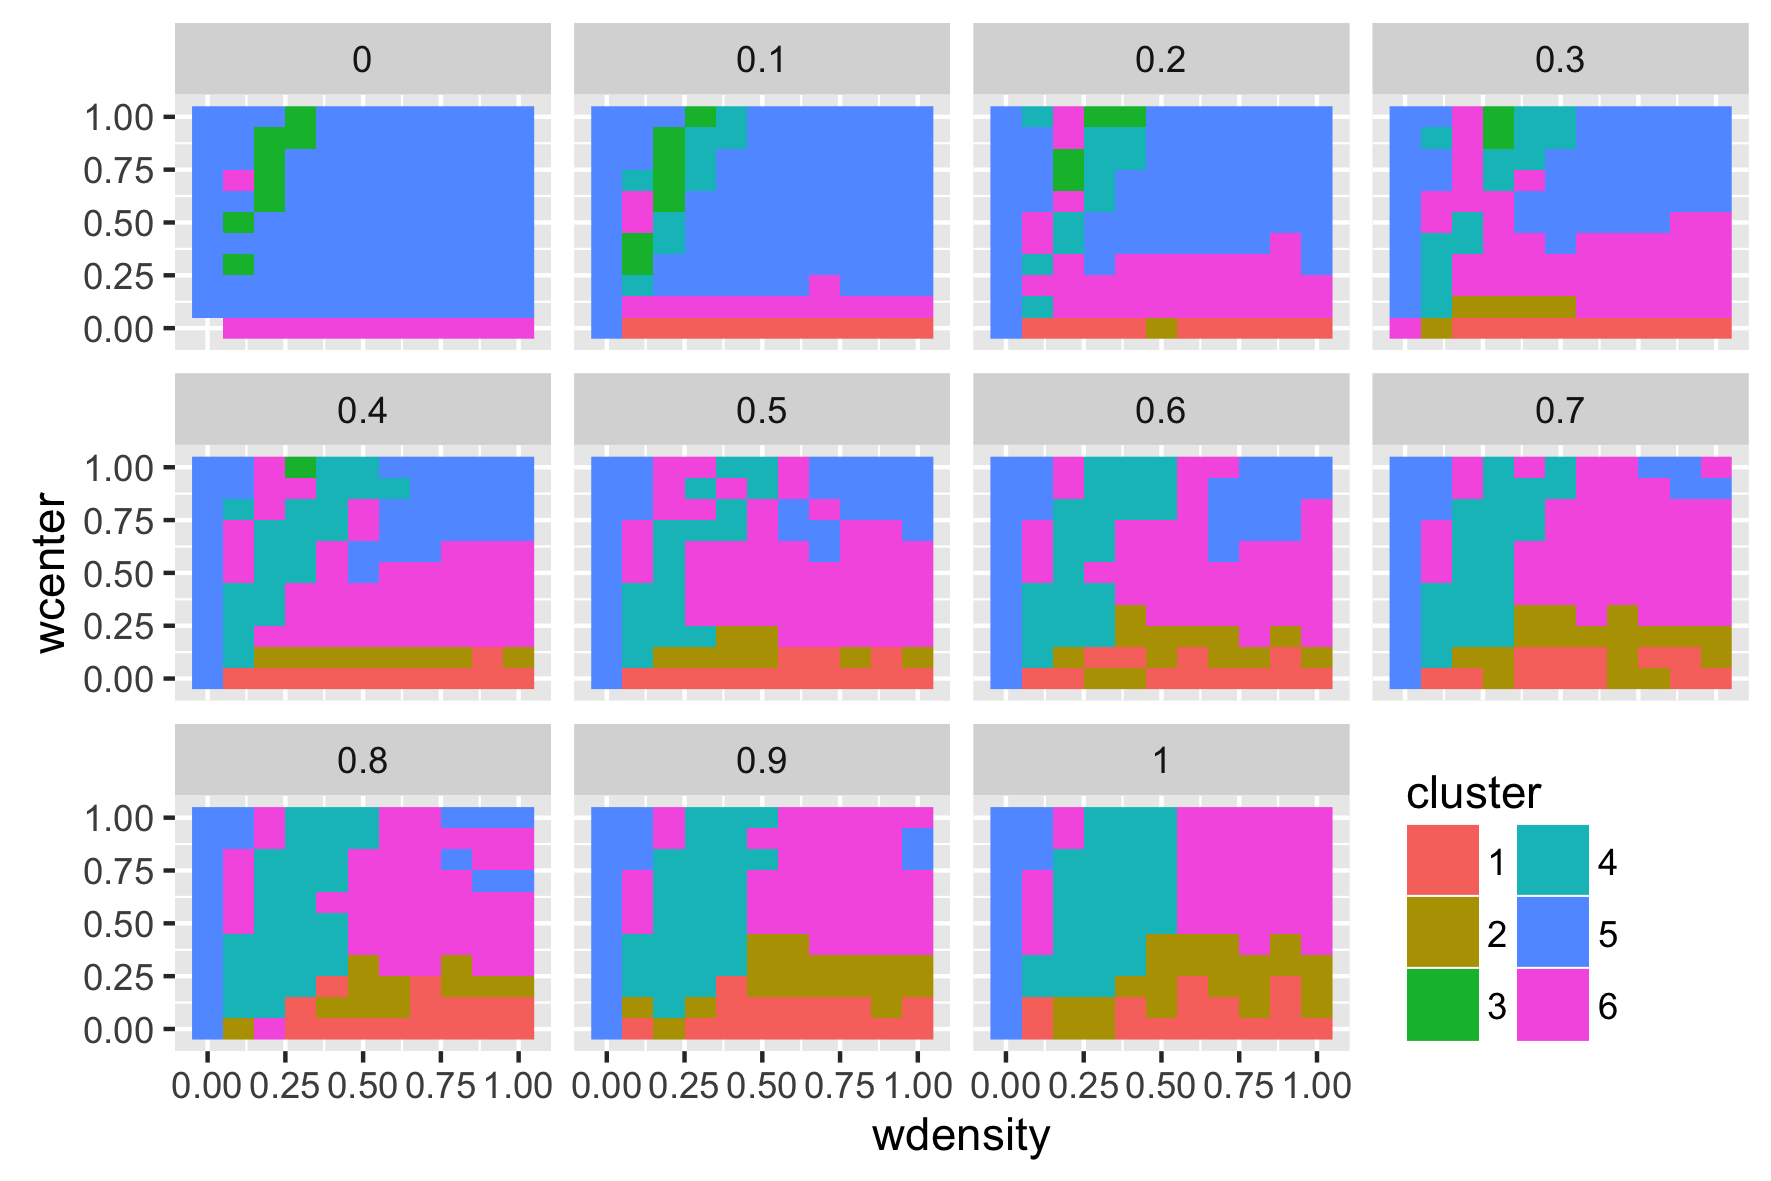
\includegraphics[width=5.9cm,height=5cm]{figures/clusters-paramfacet_valuesFALSEtheta2_k6}
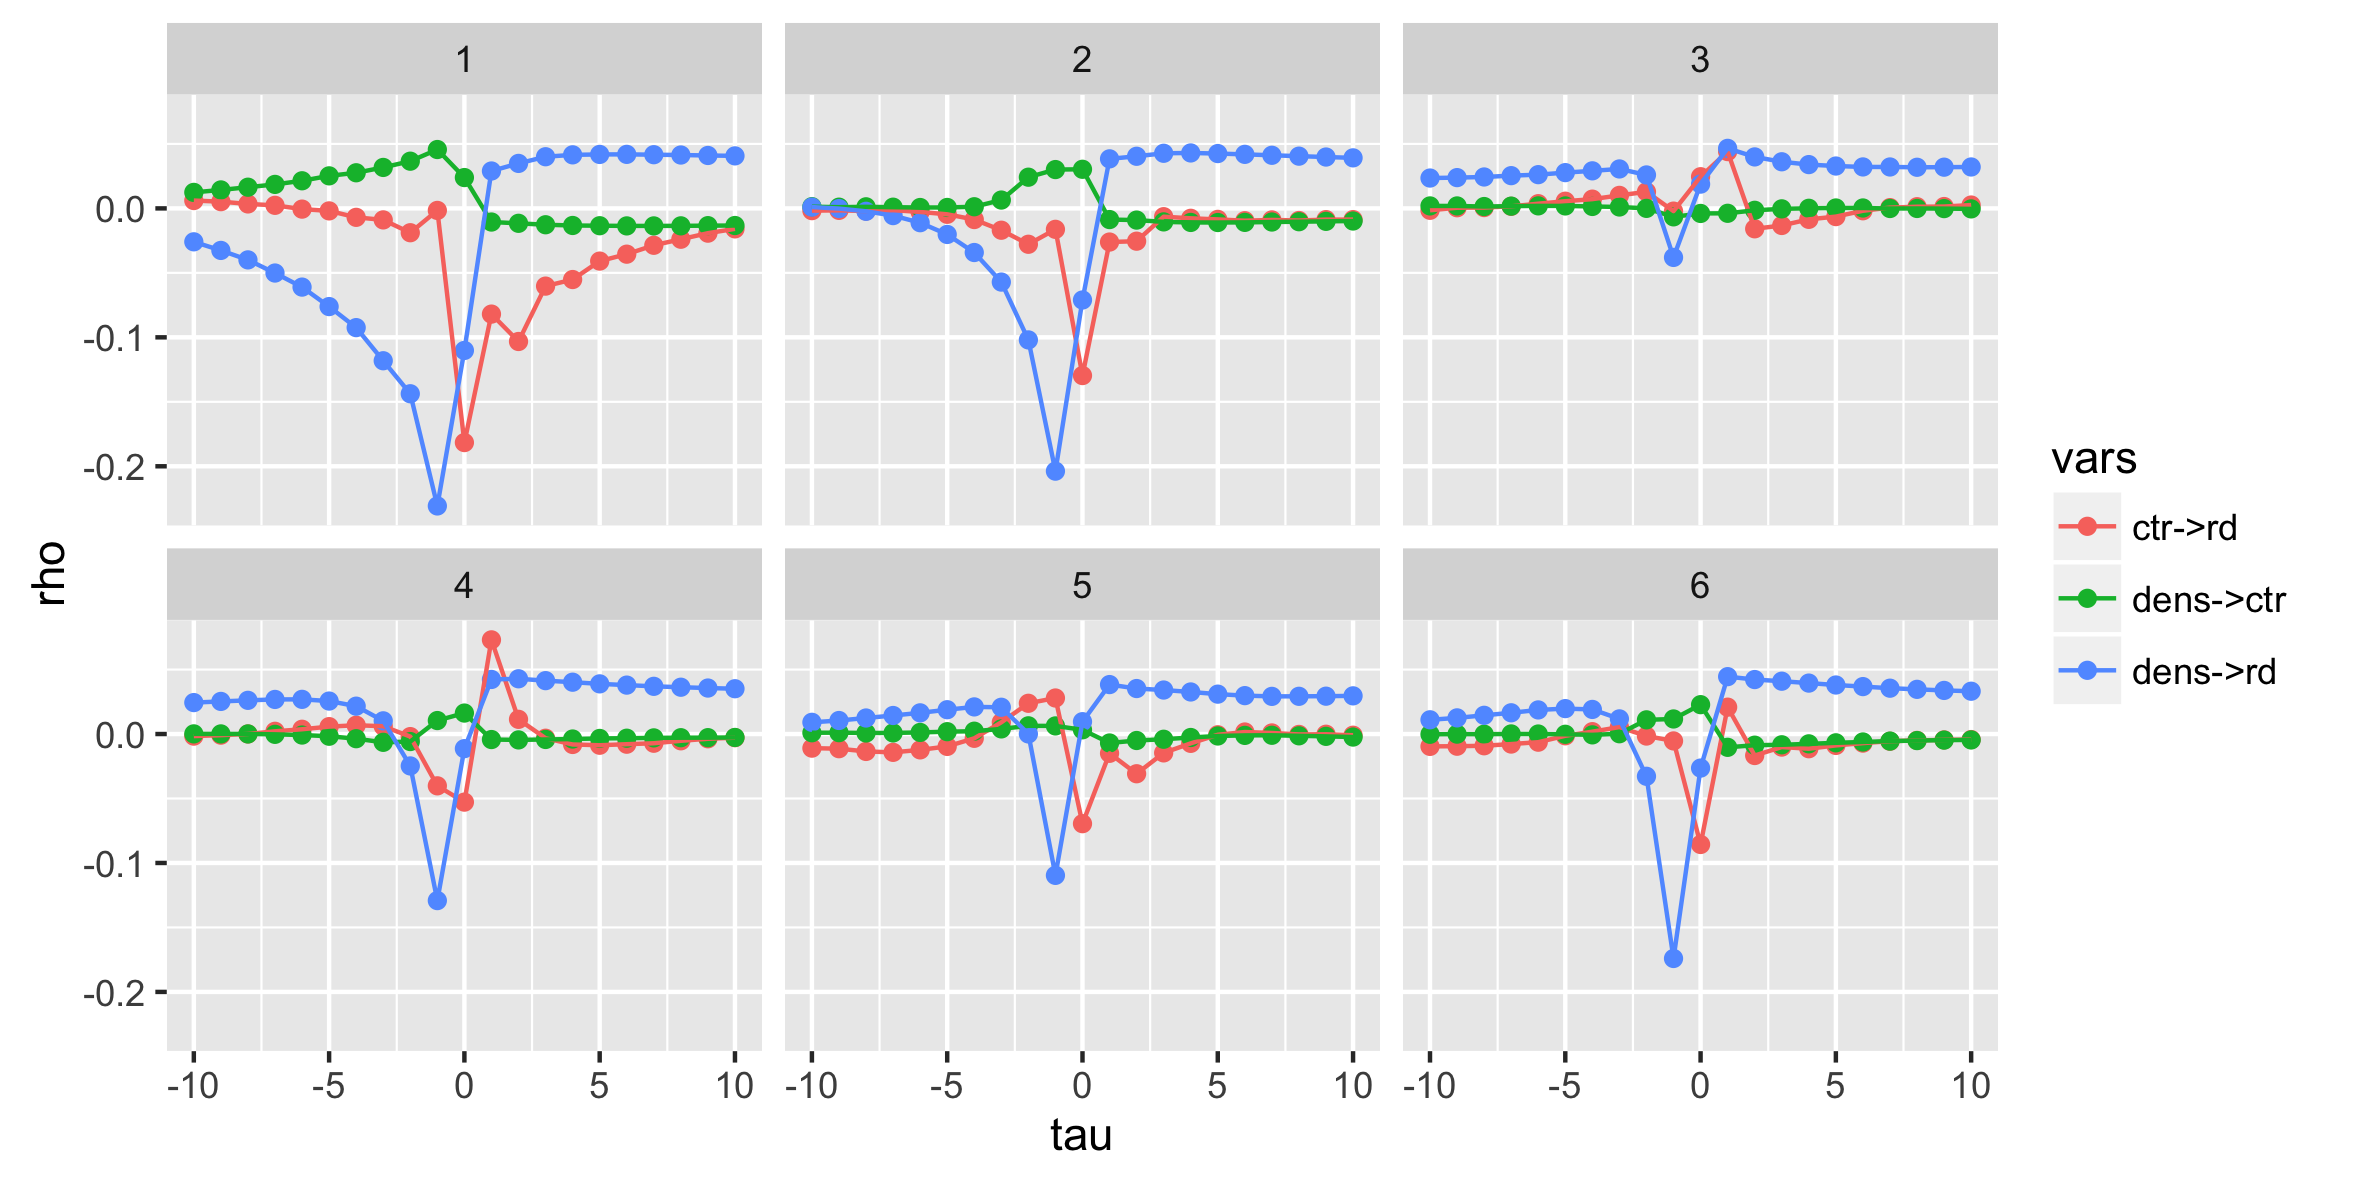
\includegraphics[width=5.9cm,height=5cm]{figures/clusters-centertrajs-facetclust_valuesFALSEtheta2_k6}
\caption{\textbf{Identification de régimes d'interactions} \textbf{(Haut Gauche)} Variance inter-cluster comme fonction du nombre de clusters. \textbf{(Haut Milieu)} Dérivée de la variance inter-cluster. \textbf{(Haut Droite)} \emph{Features} dans un plan principal (81\% de variance expliquée par les deux premières composantes) \textbf{(Bas Gauche)} Diagramme de phase des régimes dans l'espace $(w_{d},w_{c},w_{r})$, $w_r$ variant entre les différents sous-diagrammes de $(w_{d},w_{c}$. \textbf{(Bas Droite)} Trajectoires correspondantes des centroïdes.}
\label{fig:clustering}
\end{figure*}
%%%%%%%%%%%%%%%



Cette méthode doit dans un premier temps être testée et partiellement validée, ce que nous proposons de faire sur des données synthétiques, méthode qui permet une connaissance plus fine des comportements des modèles~\cite{raimbault2016generation}. En écho à l'exemple des relations entre réseaux de transport et territoires qui a permis d'introduire notre problématique précédemment, nous proposons de générer des configurations urbaines stylisées dans lesquelles réseau et densité s'influencent mutuellement, et pour lesquelles les causalités ne sont pas évidents \emph{a priori} étant donné les paramètres du modèle génératif. \cite{raimbault2014hybrid} décrit et explore un modèle simple de morphogenèse urbaine (modèle RBD) répondant parfaitement à ces contraintes. En effet, les variables explicatives de la croissance urbaine, les processus d'extension du réseau et le couplage entre densité urbaine et réseau ne sont pas trop complexes. Cependant, hormis dans des cas extrêmes (par exemple lorsque la distance au centre détermine la valeur foncière uniquement, le réseau dépendra de manière causale de la densité, ou lorsque la distance au réseau seule compte, la causalité sera inversée), les régimes mixtes n'exhibent pas de causalités évidentes : c'est donc un parfait cas pour tester si la méthode est capable d'en détecter. Nous utilisons une implémentation adaptée\footnote{disponible sur le dépôt ouvert du projet à\\\texttt{https://github.com/JusteRaimbault/CityNetwork/tree/master/Models/Simple/ModelCA}} du modèle initial, permettant de capturer les valeurs des variables étudiées pour chaque patch et à chaque pas de temps et de calculer les correlations retardées entre variables au sein du modèle. Nous explorons une grille de l'espace des paramètres du modèle RBD, faisant varier les paramètres de poids de la densité, de la distance au centre et de la distance au réseau\footnote{Le modèle fonctionne de la façon suivante : une valeur des patches est déterminée par la moyenne pondérée de ces différentes variables explicatives, valeur qui détermine la croissance de nouveaux patches à l'instant suivant.}, que l'on note respectivement $(w_{d},w_{c},w_{r})$, dans $\left[0;1\right]$ avec un pas de 0.1. Les autres paramètres sont fixés à leur valeurs par défaut données par \cite{raimbault2014hybrid}. Pour chaque valeur des paramètres, nous procédons à $N=100$ répétitions ce qui est suffisant pour une bonne convergence des indicateurs. Les explorations sont effectuées via le logiciel OpenMole~\cite{reuillon2013openmole}, le grand nombre de simulations (1,330,000) nécessitant l'utilisation d'une grille de calcul. Nous calculons sur l'ensemble des patches les corrélations retardées par estimateur de Pearson non biaisé entre les variations des variables suivantes\footnote{Calculer les corrélations sur les variables directement n'a pas de sens puisque leur valeur n'en a pas en absolu.} : densité locale, distance au centre et distance au réseau. La Fig.~\ref{fig:exrdb} montre le comportement de $\rho_{\tau}$ pour chaque couple de variable (non dirigé, $\tau$ prenant des valeurs négatives et positives), pour les combinaisons des valeurs extrêmes des paramètres. On peut voir déjà différents régimes émerger : par exemple, $(1,0,1)$ conduit à une causalité de la densité sur la distance au centre avec un retard 1, et une causalité négative de la densité sur la distance au réseau avec le même retard, tandis que distance au centre et au réseau sont corrélés de manière synchrone. Afin d'étudier ces comportements de manière systématique, nous proposons d'identifier des régimes de manière endogène, en procédant à un apprentissage non-supervisé. Nous appliquons une classification des \emph{k-means}, robuste à la stochasticité (5000 répétitions), avec les points caractéristiques (\emph{features}) suivants : pour chaque couple de variable, $\textrm{argmax}_{\tau} \rho_{\tau}$ et $\textrm{argmin}_{\tau} \rho_{\tau}$ si la valeur correspondante est telle que $\frac{\rho_{\tau}-\bar{\rho}_{\tau}}{\left|\bar{\rho}_{\tau}\right|} > \theta$ avec $\theta$ paramètre de seuil, 0 sinon. L'inclusion des \emph{features} supplémentaires des valeurs de $\rho_{\tau}$ n'influence pas significativement les résultats, celles-ci n'ont pas été prises en compte pour réduire la dimension. Le choix du nombre de clusters $k$ est en général épineux dans ce genre de problème~\cite{hamerly2003learning}, dans notre cas le système possède une structure agréable : les courbes de la proportion de variance inter-cluster et de sa dérivée en Fig.~\ref{fig:clustering}, en fonction de $k$ pour différentes valeurs de $\theta$, présentent une transition pour $\theta = 2$, ce qui donne pour cette courbe une rupture à $k=5$. Un examen visuel des clusters dans un plan principal confirme la bonne qualité de la classification pour ces valeurs. Une classe correspond alors à un \emph{régime de causalité}, dont nous pouvons représenter le diagramme de phase en fonction des paramètres du modèle, ainsi que les trajectoires des centres des clusters (calculées comme barycentre dans l'espace complet initial) en Fig.~\ref{fig:clustering}. Le comportement obtenu est particulièrement intéressant : les régions du diagramme correspondant aux régimes sont clairement délimitées et connexes. Par exemple, on observe l'émergence du régime 6 où la distance au réseau cause fortement la densité de manière négative, mais la distance au centre cause la distance au réseau, régime dont l'étendu maximale sur $(w_d,w_r)$ est pour une valeur intermédiaire $w_r=0.7$. Ainsi, pour maximiser l'impact du réseau sur la densité, il ne faut pas maximiser le poids correspondant, ce qui peut paraître contre-intuitif en premier abord : cela illustre l'intérêt de la méthode dans le cas de relations circulaires difficiles à démêler a priori. Le régime 5, où la distance au réseau influence la densité de la même manière, mais la relation entre distance au centre et route est inversée, est tout aussi intéressant, et est prédominant dans les faibles $w_r$. Le régime 1, extrême, correspond à une situation isolée dans laquelle la distance au centre n'importe pas : cet aspect domine alors totalement les autres processus d'interaction entre densité et réseau. Cette application sur données synthétique démontre ainsi d'une part la robustesse de la méthode vu la cohérence des régimes obtenus, et constitue aussi une qualification beaucoup plus précise des comportements du modèle que celle réalisée dans l'article initial. Dans ce cas précis, il peut s'agir d'un instrument de connaissance des relations entre réseaux et territoires en lui-même, permettant le test d'hypothèses ou la comparaison de processus dans le modèle stylisé.







%%%%%%%%%%%%%%%
\subsection{Cas d'étude}


\subsubsection{Contexte}

Nous proposons une application sur un cas d'étude réel, toujours lié aux relations entre réseaux de transport et territoires. La région métropolitaine de Paris est en train de connaître de grandes mutations, avec la mise en place d'une gouvernance métropolitaine et de nouvelles infrastructures de transport par exemple. La construction d'un réseau de métro en rocade permettant des liaisons de banlieue à banlieue est un besoin ancien, et a mené à plusieurs propositions sur lesquelles se sont opposés l'Etat et la Région au tournant des années 2010~\cite{desjardins2010bataille}. Le projet Arc Express~\cite{stif2007arc}, porté par la Région et plus axé sur une égalité des territoires, contrastait avec les propositions initiales de Réseau du Grand Paris visant à relier des ``clusters d'excellence'' en dépit d'un possible effet tunnel. La solution finalement adoptée (voir le dernier schéma directeur \cite{sdrif2013}) est un compromis et permet un rééquilibrage est-ouest de l'accessibilité~\cite{beaucire2013grand}. Nous proposons d'étudier les relations entre différentiel d'accessibilité pour chaque projet, et variables liées au foncier (transactions immobilières) et socio-économiques. En effet, les liens entre nouvelles lignes et évolution du foncier sont parfois remarquables~\cite{damm1980response}.



%%%%%%%%%%%%%%%
\begin{figure*}[h]
\centering
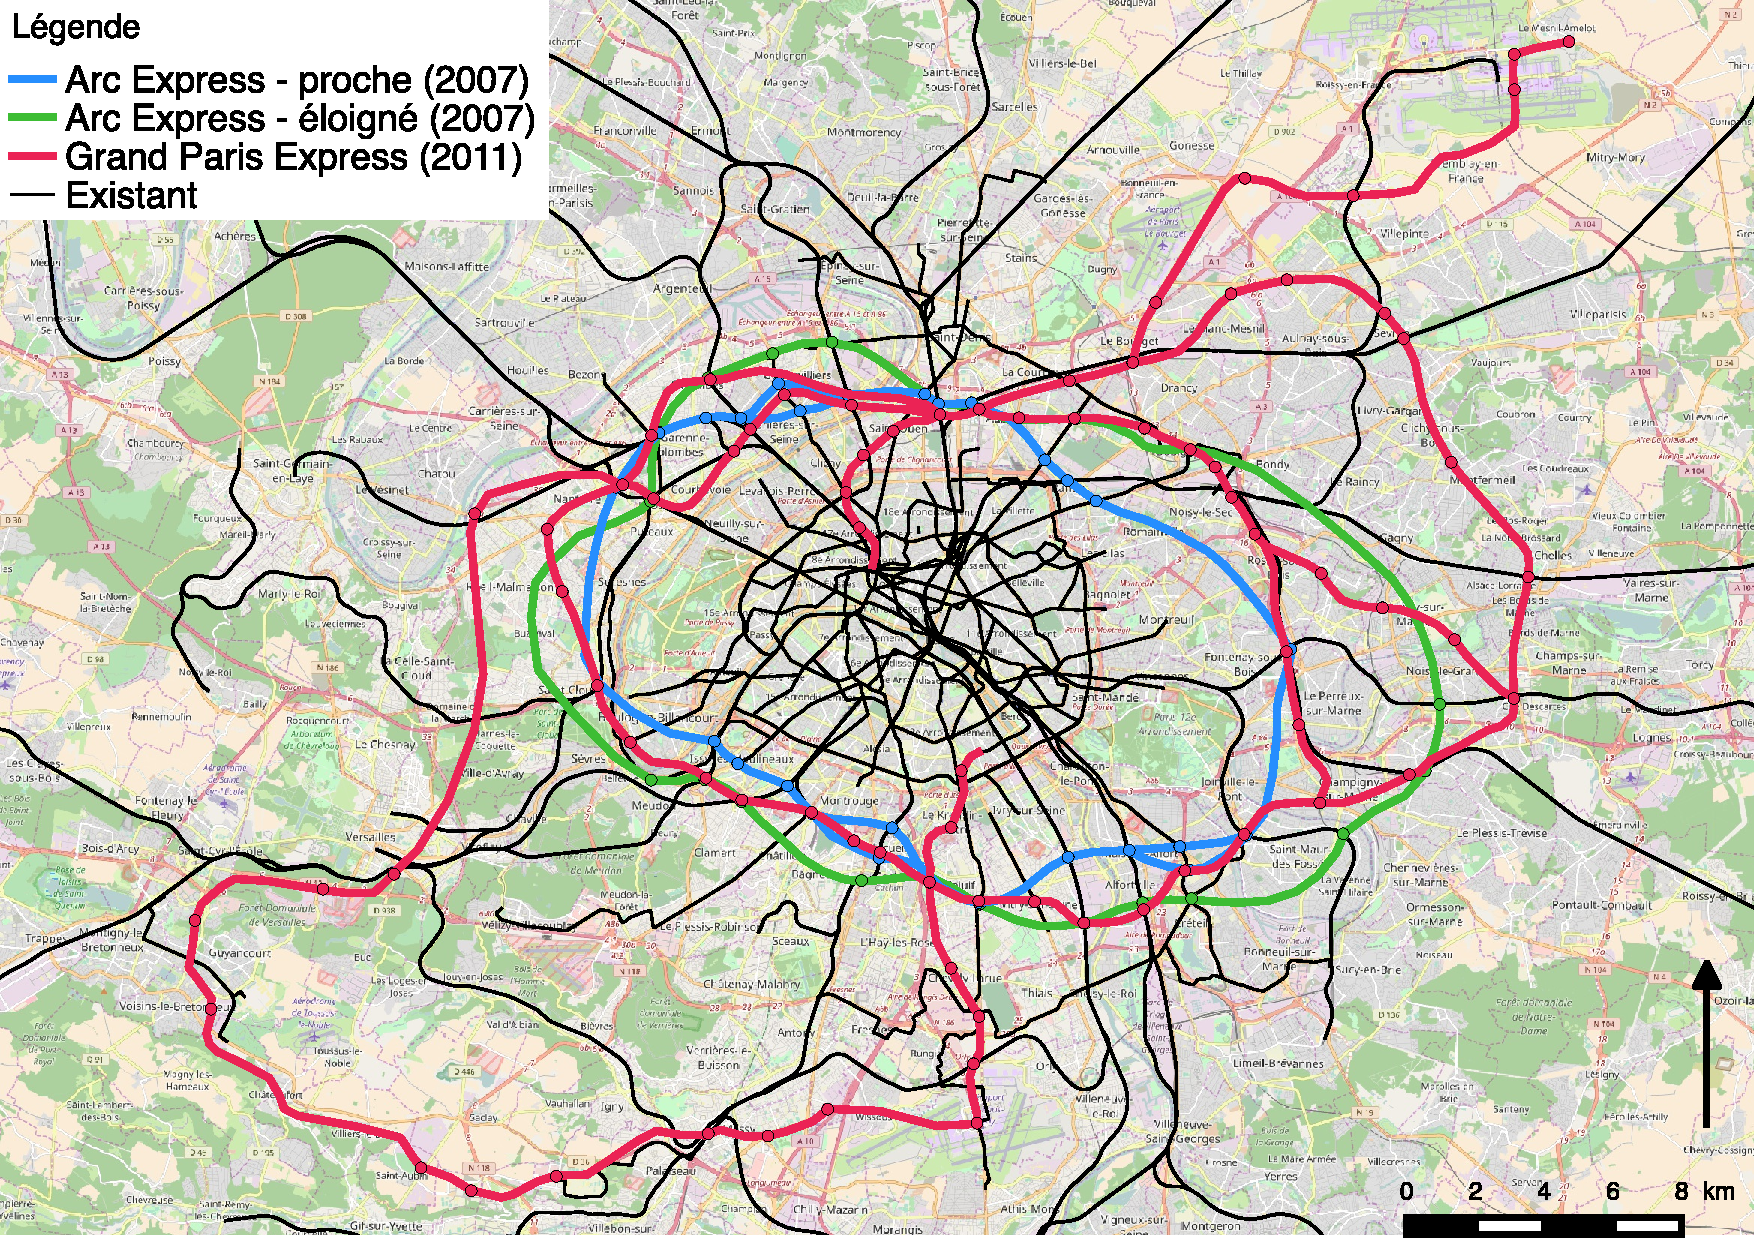
\includegraphics[width=12cm]{figures/reseaux}
\caption{\textbf{Projets de transport successifs de la métropole du Grand Paris.} Nous montrons les deux alternatives du projet Arc Express porté par la région, et le Grand Paris Express (GPE) porté par l'état. Le Réseau du Grand Paris, précurseur du GPE, n'est pas montré ici pour des raisons de visibilité à cause de sa proximité avec celui-ci.}
\label{fig:projects}
\end{figure*}
%%%%%%%%%%%%%%%

\subsubsection{Données}

Les données des transactions immobilières sont fournies par la base BIENS (Chambre des Notaires d'Ile de France, base propriétaire). Le nombre de transactions utilisables après nettoyage est de 862360, se répartissant sur l'ensemble des IRIS, pour une plage temporelle couvrant de 2003 à 2012 incluses. Les données par IRIS pour population et revenu (revenu médian et indice de Gini) proviennent de l'INSEE. Les données de réseau ont été vectorialisées à partir des cartes des projets (voir Fig.~\ref{fig:projects} pour les projets). Les temps de trajets sont calculés par transport en commun uniquement, avec des valeurs standard pour les vitesses moyennes des différents modes (RER 60km.h\textsuperscript{-1}, Transilien 100km.h\textsuperscript{-1}, Metro 30km.h\textsuperscript{-1}, Tramway 20km.h\textsuperscript{-1}). La matrice des temps est calculée depuis l'ensemble des centroïdes des IRIS vers l'ensemble des centroïdes des communes. Ceux-ci sont reliés au réseau par des connecteurs à la gare la plus proche, de vitesse 50km.h\textsuperscript{-1} (trajet en voiture). Les analyses sont implémentées intégralement en langage R~\cite{rcoreteam} et l'ensemble des données, du code source et des résulats sont disponibles sur un dépôt git ouvert\footnote{A l'adresse\\\texttt{https://github.com/JusteRaimbault/CityNetwork/tree/master/Models/SpatioTempCausality/GrandParis}. Les données de la base BIENS ne sont fournies que de manière agrégée à l'IRIS et pour les variables de prix et de crédit, pour des raisons de fermeture contractuelle de la base brute.}.


\subsubsection{Résultats}


% note : étude de l'accessibilité pondérée : pas conclusif au regard des réseaux de transports car pas sensible à un changement de réseau, majoritairement influencé par les variables territoriales.

% low decay increase absolute correlation (expected ?)



%%%%%%%%%%%%%%%
\begin{figure*}[h]
%\centering
\hspace{-1cm}
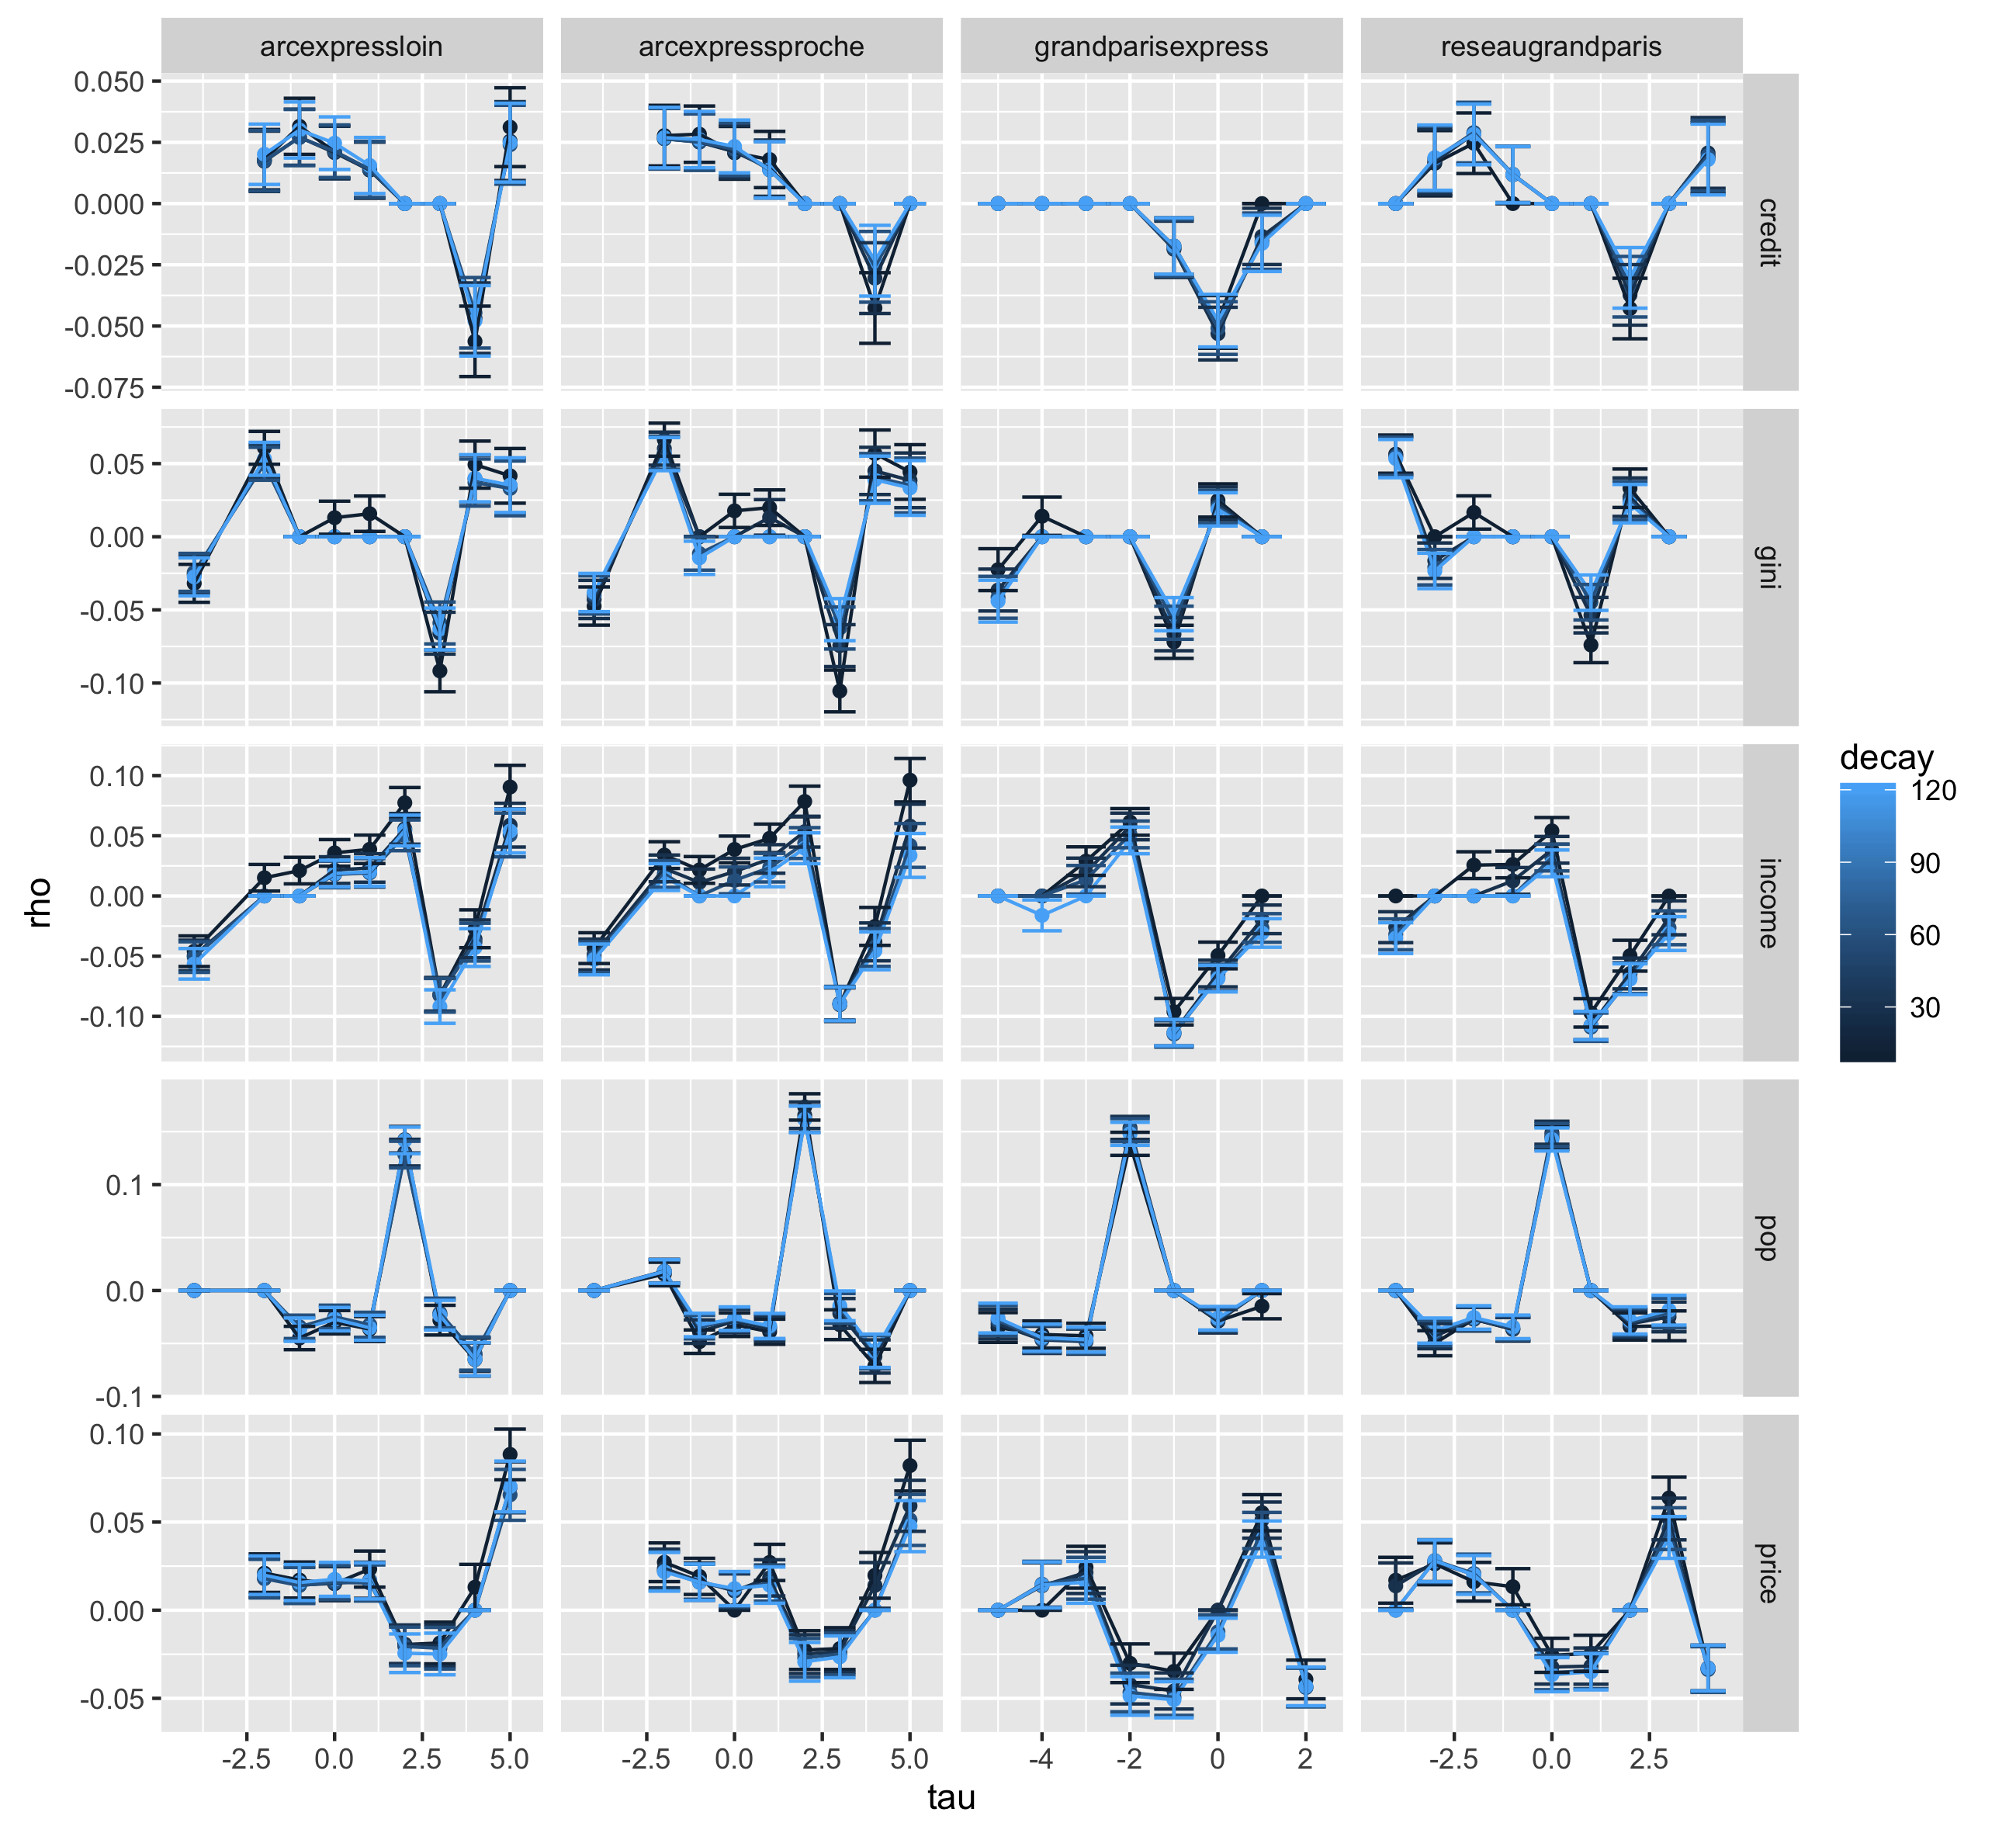
\includegraphics[width=14cm]{figures/laggedcorrs_times_allvars}
\caption{\textbf{Corrélations retardées empiriques.} Les graphiques donnent la valeur de la correlation entre le différentiel d'accessibilité en temps de trajet moyen $\Delta T$ pour chaque projet (en colonnes) et le différentiel des différentes variables socio-economiques et de transactions immobilières (en lignes), pour différentes valeurs du paramètre d'atténuation (\texttt{decay}). Les barres d'erreur donnent l'intervalle de confiance à 95\%.}
\label{fig:empiricalres}
\end{figure*}
%%%%%%%%%%%%%%%


Nous calculons pour chaque projet, le différentiel $\Delta T_i$ d'accessibilité en temps moyen de trajet à partir de chaque IRIS en comparaison à celui dans le réseau sans le projet, défini par $T_i = \sum_k \exp{-t_{ik}/t_0}$ avec $k$ communes, $t_{ik}$ temps de trajet, et $t_0$ paramètre d'atténuation. A chaque projet est associée une date\footnote{2006 pour Arc Express, 2008 pour le Réseau du Grand Paris, 2010 pour le Grand Paris Express}, correspondant environ à l'année d'annonce mature du projet, restant toutefois arbitraire car difficile d'une part à déterminer précisément, un projet n'émergeant pas d'un coup du jour au lendemain, et d'autre part pouvant correspondre à des réalités différentes d'apprentissage du projet par les différents agents économiques (nous faisons donc l'hypothèse réductrice mais nécessaire d'une diffusion sur la majorité des agents dans un temps inférieur à l'année). Nous étudions les corrélations décalées de cette variable avec les variations $\Delta Y_{ij}$ des variables socio-économiques suivantes : population, revenu médian, indice de Gini des revenus, prix moyen des transactions immobilières et montant moyen des crédits immobiliers. Un test de Fisher est effectué pour chaque estimation, et la valeur est fixée nulle si celui-ci n'est pas significatif ($p<0.05$ de manière classique). L'étude avec accessibilité généralisées au sens de Hansen a également été menée mais moins intéressante car très peu sensible à la composante mobilité (réseau et atténuation) par rapport aux variables elle-même, informe uniquement sur des relations entre celles-ci et n'est donc pas présentée ici. Nous présentons en Fig.~\ref{fig:empiricalres} les résultats pour l'ensemble des réseaux et variables. Il est remarquable tout d'abord de noter l'existence d'effets significatifs pour l'ensemble des variables. Des valeurs plus basses du paramètre $t_0$ donnent des corrélations plus fortes en valeur absolue, révélant une possible plus grande importance de l'accessibilité locale sur les dynamiques territoriales. Le comportement de la population montre un pic très détaché correspondant à 2008, laissant supposer un impact du plus vieux projet d'Arc Express sur la croissance de la population, l'effet des autres projets serait alors fallacieux de par leur proximité dans les grands tronçons : cela impliquerait que les zones où ils diffèrent fondamentalement comme le Plateau de Saclay ne soient que très peu sensibles au projet de transport, ce qui confirmerait l'aspect artificiel planifié du développement de ce territoire. Concernant les revenus, on observe un comportement similaire mais négatif, ce qui impliquerait un appauvrissement lié à l'augmentation de l'accessibilité, mais qui semble toutefois s'accompagner d'une baisse des inégalités. Enfin, comme attendu les prix immobiliers sont tirés par l'arrivée potentielle des nouveaux réseaux, effet qui disparait à deux ans pour le Grand Paris Express, suggérant une bulle immobilière passagère. Nous démontrons ainsi l'existence de liens de correlations retardées complexes qu'on nomme causalités en ce sens, entre dynamiques territoriales et dynamiques anticipées des réseaux. Une compréhension plus fine des processus à l'oeuvre est au delà de la portée de cet article, car supposerait des études de terrain qualitatives, des études de cas ciblées, etc. Cet exemple illustre cependant le caractère opérationnel de notre méthode sur un cas d'étude réel.
 








%%%%%%%%%%%%%%%
\section{Discussion}
%%%%%%%%%%%%%%%


%%%%%%%%%%%%%%%
\subsection{Diffusion spatio-temporelle}

% STARMA, ondes, ergodicité etc.

L'application de notre approche doit être menée précautionneusement concernant le choix des  échelles, processus et objets d'étude. Typiquement, elle ne sera pas du tout adaptée à la quantification de processus spatio-temporels dont l'échelle temporelle de diffusion est de l'ordre de celle de la fenêtre d'estimation : l'hypothèse de stationnarité est basique. On peut proposer de procéder à des estimations par fenêtres glissantes, mais il faudrait ensuite élaborer une technique de correspondance spatiale pour traquer la propagation des phénomènes. Un exemple d'application concrète à l'impact thématique fort serait une caractérisation d'une composante fondamentale de la Théorie Evolutive des Villes, la diffusion hiérarchique de l'innovation entre les villes~\cite{pumain2010theorie}, en analysant les potentielles dynamiques spatio-temporelles des classifications de brevets comme celle introduite par~\cite{10.1371/journal.pone.0176310}. Il faut noter toutefois qu'il s'agit de questions méthodologiques relativement ouvertes, dont une des manifestations est le lien potentiel entre le caractère non-ergodique des systèmes urbains~\cite{pumain2012urban} et une caractérisation ondulatoire de ces processus.




%%%%%%%%%%%%%%%
\subsection{Regression Géographique Pondérée}

% lien avec GWR ?

Une autre direction de développement et d'applications potentiels se révèle en se tournant vers l'échelle plus locale, et d'explorer une hybridation avec les techniques de Regression Géographique Pondérée~\cite{brunsdon1998geographically}. La détermination par validation croisée ou Critère d'Akaike d'une portée spatiale optimale pour la performance de ce type de modèles pourrait être adaptée dans notre cas pour déterminer une échelle locale optimale sur laquelle les correlations retardées sont les plus significatives, ce qui permettrait de s'extraire du problème de la non-stationnarité prioritairement par l'aspect spatial.




%%%%%%%%%%%%%%%
\section{Conclusion}
%%%%%%%%%%%%%%%

Nous avons proposé une méthode générique de causalité de Granger sur des données territoriales, puis démontré sa potentialité et son caractère opérationnel sur données synthétiques et un cas réel. Nous postulons que l'appareillage méthodologique simple est un atout pour une certaine généralité, mais que l'application à ces cas complexes présentant des causalités circulaires a un fort potentiel de contribution à la compréhension des dynamiques de ce type de systèmes co-évolutifs.


%%%%%%%%%%%%%%%
\section*{Remerciements}

Les résultats obtenus dans la section 3.1 de cet article ont été calculés sur l'organisation virtuelle vo.complex-system.eu de l'European Grid Infrastructure (http://www.egi.eu). Nous remercions l'European Grid Infrastructure et ses National Grid Initiatives (France-Grilles en particulier) pour fournir le support technique et l'infrastructure.



%%%%%%%%%%%%%%%
%% Biblio
%%%%%%%%%%%%%%%

\bibliography{biblio,/Users/Juste/Documents/ComplexSystems/CityNetwork/Biblio/BibTeX/CityNetwork}







%%%%%%%%%%%%%%%
%% TEMPLATES
%%%%%%%%%%%%%%%

%
%
%
%\section{Section 1}
%
%\subsection{Sous-section 1}
%
%\subsubsection{Sous-sous-section 1}
%
%\begin{figure*}[h]
%   \centering  
\includegraphics[width=8cm]{grenouille.jpg}
%  \caption{\label{fig:1} Une grenouille bien verte.}
%\end{figure*}
%
%\subsection{Sous-section 2}
%
%\section{Section 2}
%
%Listes :
%\begin{itemize}
%\item ligne 1 (cf. équation \ref{eq:form1})
%\item ligne 2 (cf. équation \ref{eq:form2})
%\end{itemize}
%
%Formules :
%
%\begin{equation}
%	R = \frac{d_1}{d_2}
%	\label{eq:form1}
%\end{equation}
%
%\begin{equation}
%	\sin(\alpha) = \frac{h}{l}
%    \label{eq:form2}
%\end{equation}
%
%\begin{table*}[h!]
%\begin{center}
%\caption{\label{tab:1} Exemple de tableau}
% \scriptsize
%      \begin{tabular}{|c|c|c|c|c|}
%   \hline
%   \multirow{2}*{ Clients} & \multicolumn{2}{| c |}{Départ }  & \multicolumn{2}{| c |}{ Arrivée}\\
%   \cline{2-5}
%      & Station  & Période de Temps & Station  & Période de Temps \\\hline
%   client 1 (c1) & 3  & 2 & 1 & 4 \\\hline
%   client 2 (c2)   &   2  & 2 & 3 & 3\\\hline
%   client 3 (c3)   &   2 & 2 & 3 & 4  \\\hline
%   client 4 (c4)   &   3 & 2 & 2 & 3  \\\hline
%   client 5 (c5)   &   3 & 2 & 2 & 4  \\\hline
%  client 6 (c6)   &   2  & 4 & 3 & 5\\\hline
%   client 7 (c7)   &   3  & 3 & 2 & 6  \\\hline
%   client 8 (c8)   &   1 & 5 & 3 & 6 \\\hline
%   client 9 (c9) & 2  & 6 & 3 & 7 \\\hline
%    client 10 (c10)  &   3 & 7 & 1 & 9 \\\hline
%   client 11 (c11) & 1  & 6 & 2 & 7 \\\hline
%%\hline
%\end{tabular}
%\end{center}
%\end{table*}
%
%Exemple d'algorithme :
%
%\begin{algorithm}[h!]
%\label {algo}
% \KwData{
% $G(V,A,C,R,U)$ \; \tcc{commentaire}}
% \KwResult{
% $Paths_{Cars}, \; Relocation,\; SatisfiedDemands, Paths_{Agents}  $
% }
% initialization\;
% $Paths_{Agents} \gets \emptyset $ /* l'ensemble de chemins... */ \;
% $j \gets 1$ \;
% $costPath_j  \gets 0$ \;
% \While { $ (j \le  nb_{Veh}) \wedge (costPath_j \leq 0)  $ }
% {
% $ path_j \gets Dijkstra(G(V,A, C,R)) $ \;
%$ costPath_j \gets  Cost (path_j)$ \;
%  \ForAll { $(v^{k}_{t'},v^{i}_{t}) \in path   $}
%{
% \ForAll {$ U_{r^{i}_{t'',t''+1}} $  }
% {....
% }
%$ Paths_{Cars} \gets Paths_{Cars} \cup path_j $  \;
% }
%$j \gets j+1$ \;
% }
%$Paths_{Agents} \gets  routeAgents (Relocation ); $
% \caption{un algorithme très glouton}
%\end{algorithm}
%









\end{document}